\documentclass[tikz,border=10pt]{standalone}
\usepackage{tikz}
\usetikzlibrary{shapes.geometric, arrows.meta, positioning, calc, fit, backgrounds}
\usepackage{amsmath,amssymb}
\usepackage{xcolor}

% Unified Academic Color Palette
\definecolor{cInput}{RGB}{235, 248, 255}
\definecolor{bInput}{RGB}{49, 130, 206}

\definecolor{cTrans}{RGB}{240, 249, 255}
\definecolor{bTrans}{RGB}{43, 108, 176}

\definecolor{cGCN}{RGB}{230, 255, 250}
\definecolor{bGCN}{RGB}{49, 151, 149}

\definecolor{cRecurr}{RGB}{250, 245, 255}
\definecolor{bRecurr}{RGB}{128, 90, 213}

\definecolor{cHead}{RGB}{255, 245, 245}
\definecolor{bHead}{RGB}{229, 62, 62}

\definecolor{cFusion}{RGB}{254, 252, 191}
\definecolor{bFusion}{RGB}{214, 158, 46}

\definecolor{cGray}{RGB}{247, 250, 252}
\definecolor{bGray}{RGB}{160, 174, 192}

\definecolor{tDark}{RGB}{26, 32, 44}
\definecolor{tMuted}{RGB}{74, 85, 104}

\begin{document}
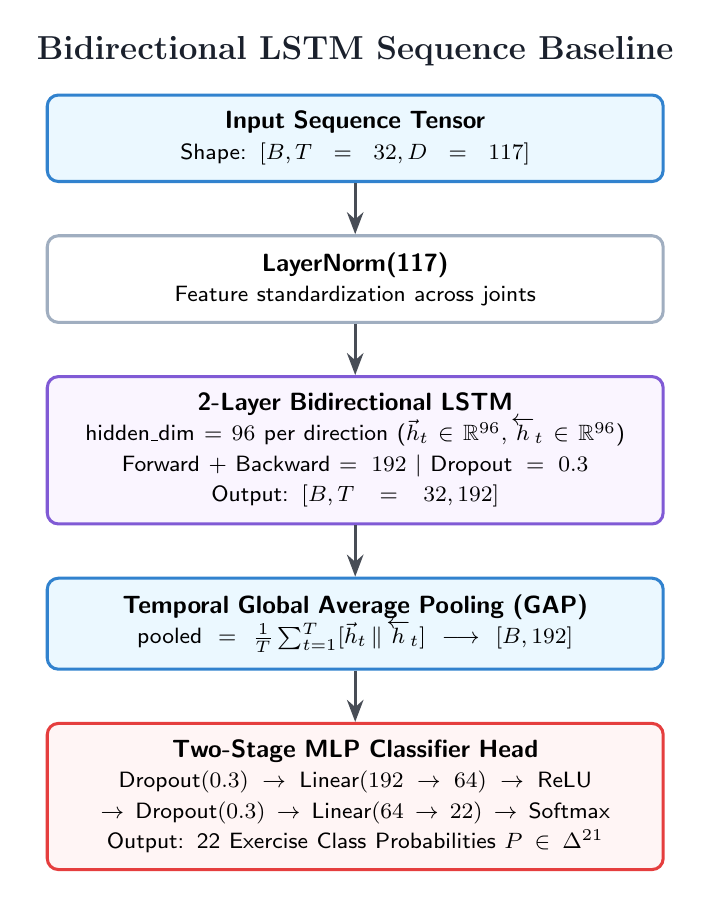
\begin{tikzpicture}[
    font=\sffamily\small,
    >=Stealth,
    node distance=0.65cm,
    block/.style={
        draw=#1,
        line width=1.1pt,
        rounded corners=4pt,
        align=center,
        inner sep=6pt
    },
    arrow/.style={->, line width=1.1pt, color=tDark!80}
]

\node[font=\bfseries\large, text=tDark] (title) at (0, 1.1) {Bidirectional LSTM Sequence Baseline};

\node[block=bInput, fill=cInput, text width=7.4cm] (input) at (0, 0) {
    \textbf{Input Sequence Tensor}\\
    {\footnotesize Shape: $[B, T=32, D=117]$}
};

\node[block=bGray, fill=white, text width=7.4cm, below=of input] (norm) {
    \textbf{LayerNorm(117)}\\
    {\footnotesize Feature standardization across joints}
};

\node[block=bRecurr, fill=cRecurr, text width=7.4cm, below=of norm] (bilstm) {
    \textbf{2-Layer Bidirectional LSTM}\\
    {\footnotesize $\text{hidden\_dim} = 96$ per direction ($\vec{h}_t \in \mathbb{R}^{96}, \overleftarrow{h}_t \in \mathbb{R}^{96}$)}\\
    {\footnotesize Forward + Backward $= 192$ \textbar{} $\text{Dropout} = 0.3$}\\
    {\footnotesize Output: $[B, T=32, 192]$}
};

\node[block=bInput, fill=cInput, text width=7.4cm, below=of bilstm] (gap) {
    \textbf{Temporal Global Average Pooling (GAP)}\\
    {\footnotesize $\text{pooled} = \frac{1}{T}\sum_{t=1}^T [\vec{h}_t \,\|\, \overleftarrow{h}_t] \longrightarrow [B, 192]$}
};

\node[block=bHead, fill=cHead, text width=7.4cm, below=of gap] (head) {
    \textbf{Two-Stage MLP Classifier Head}\\
    {\footnotesize $\text{Dropout}(0.3) \to \text{Linear}(192 \to 64) \to \text{ReLU}$}\\
    {\footnotesize $\to \text{Dropout}(0.3) \to \text{Linear}(64 \to 22) \to \text{Softmax}$}\\
    {\footnotesize Output: 22 Exercise Class Probabilities $P \in \Delta^{21}$}
};

\draw[arrow] (input) -- (norm);
\draw[arrow] (norm) -- (bilstm);
\draw[arrow] (bilstm) -- (gap);
\draw[arrow] (gap) -- (head);

\end{tikzpicture}
\end{document}
